% =============================================================================
% APPENDIX — content migrated from the main paper to save space.
% Sections in this file (suggested ordering — re-letter as needed when merging
% with any existing appendix material):
%
%   A.  Corpus Details
%       A.1  Topic-category distribution and per-property statistics
%   B.  Algorithmic Details
%       B.1  Single-function FIM target selection (Algorithm 1)
%       B.2  Program dependency graph: call resolution
%       B.3  Complexity score: caps and weights
%       B.4  Inferability score: component formulas
%       B.5  Difficulty Δ, one-sided Gaussian penalty ρ, and hard filters
%       B.6  Multi-function group score
%       B.7  Chain-of-thought prompt template
%   C.  Consistency Across Model Sizes
%   D.  Extended Behavioral Analysis (overflow from Section 5)
%       D.1  Full trajectory metrics
%       D.2  Iterate-and-verify: action-type distribution
%       D.3  Failure-mode breakdown (outcome-distribution figure)
%       D.4  No-patch mode: mechanism
%       D.5  Multi-file tasks
%       D.6  A concrete contrast (scikit-learn-26323)
%
% Behavioral analysis on SWE-Bench-Lite (already in the previous appendix)
% should follow these sections under the existing
% \label{app:behavior_lite}; it is left in place.
% =============================================================================

\section{Corpus Details}
\label{app:data}

This appendix expands on the data collection summary in
Section~\ref{sec:method:data}. The full repository list, license inventory,
and commit hashes will be released; here we report category coverage and
per-property statistics.

% -----------------------------------------------------------------------------
% Figure (categories) and Table (corpus stats) — moved from main paper
% -----------------------------------------------------------------------------
\begin{figure}[h]
\centering
\begin{minipage}[t]{0.50\linewidth}
  \centering
  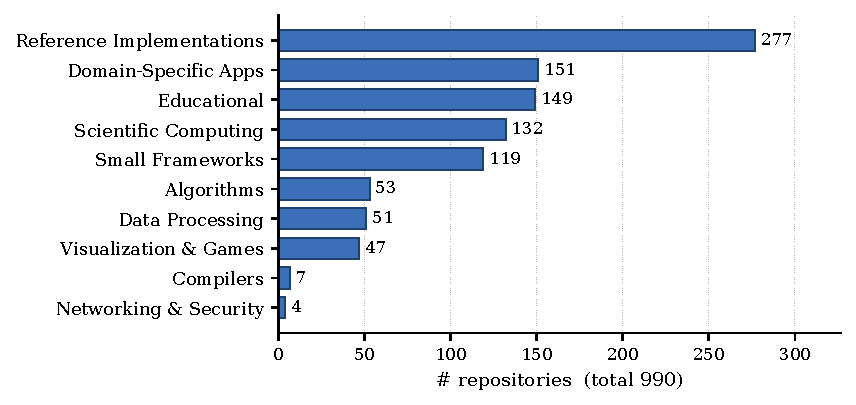
\includegraphics[width=\linewidth]{figs/dataset_categories.pdf}
  \caption{Distribution of the 990 source repositories across
  ten topic categories. The corpus is dominated by reference
  implementations, scientific computing, and small frameworks; compilers
  and networking/security tails remain by design to maintain coverage
  diversity.}
  \label{fig:dataset_categories}
\end{minipage}\hfill
\begin{minipage}[t]{0.46\linewidth}
  \vspace{0pt}
  \centering
  \caption{Mid-training corpus statistics after decontamination
  and quality filtering. Token counts are reported with the Qwen2.5-Coder
  tokenizer.}
  \label{tab:dataset}
  \scriptsize
  \setlength{\tabcolsep}{4pt}
  \begin{tabular}{lr}
  \toprule
  Property & Value \\
  \midrule
  Source GitHub repositories                       & $990$ \\
  Topic categories                                 & $10$ \\
  Filtered self-contained Python files             & $\approx 78\mathrm{K}$ \\
  Total lines of Python code                       & $\approx 33\mathrm{M}$ \\
  Mean LoC per file                                & \textcolor{red}{$\approx 425$} \\
  Mid-training token budget                        & $\approx 3\mathrm{B}$ \\
  \midrule
  Single-function FIM targets                      & \textcolor{red}{$\approx 412\mathrm{K}$} \\
  Multi-function targets ($k{=}2$)                 & \textcolor{red}{$\approx 96\mathrm{K}$} \\
  Multi-function targets ($k{=}3$)                 & \textcolor{red}{$\approx 31\mathrm{K}$} \\
  Mean target LoC                                  & \textcolor{red}{$\approx 38$} \\
  Targets with Gemini-3 CoT                        & \textcolor{red}{$100\%$} \\
  \midrule
  SWE-Bench source-repo overlap                    & $0$ \\
  Commit cutoff                                    & before earliest SWE-Bench base \\
  License inventory                                & permissive only \\
  \bottomrule
  \end{tabular}
\end{minipage}
\end{figure}

% =============================================================================
\section{Algorithmic Details}
\label{app:algo}

This appendix collects the full algorithmic details that are summarized
in Section~\ref{sec:method:selection}.

\subsection{Single-Function FIM Target Selection}
\label{app:algo:single}

Algorithm~\ref{alg:selection} summarizes the per-file pipeline that
produces single-function FIM targets. It composes the program dependency
graph (Section~\ref{sec:method:pdg}), the complexity score $\hat{H}$
(Section~\ref{sec:method:complexity}), the inferability score $\hat{I}$
(Section~\ref{sec:method:inferability}), the difficulty penalty $\rho$
(Appendix~\ref{app:algo:penalty}), and hard filters described below.

\begin{algorithm}[h]
\caption{Single-function FIM target selection for one file.}
\label{alg:selection}
\begin{algorithmic}[1]
  \Require Source file $s$; thresholds $\tau_d, \tau_{\mathrm{FIM}}, \tau_{\hat H}$
  \State $T \gets \mathrm{ParseAST}(s)$
  \State $\mathcal{V}, \mathcal{E}_{\mathrm{call}}, \mathcal{E}_{\mathrm{sib}} \gets \mathrm{BuildPDG}(T)$
        \Comment{Section~\ref{sec:method:pdg}}
  \State $\mathcal{C} \gets \emptyset$
  \For{each $v \in \mathcal{V}$}
    \If{$v$ is a dunder method \textbf{or} $\mathrm{LoC}(v) \notin [10, 200]$}
      \State \textbf{continue}
    \EndIf
    \State Compute $\hat{H}(v)$ and $\hat{I}(v)$
          \Comment{Eqs.~\eqref{eq:complexity}, \eqref{eq:inferability}}
    \If{$\hat{H}(v) < \tau_{\hat H}$} \textbf{continue} \EndIf
    \State $\Delta(v) \gets \max(0, \hat{H}(v)-\hat{I}(v)) / (\hat{H}(v)+\epsilon)$
    \State $\mathrm{FIM}(v) \gets \dfrac{\hat{H}(v)\,\hat{I}(v)}{\hat{H}(v)+\hat{I}(v)+\epsilon}\cdot \rho(\Delta(v))$
    \If{$\mathrm{FIM}(v) \ge \tau_{\mathrm{FIM}}$}
      \State $\mathcal{C} \gets \mathcal{C} \cup \{v\}$
    \EndIf
  \EndFor
  \State \Return $\mathcal{C}$ \Comment{ranked by $\mathrm{FIM}$ descending}
\end{algorithmic}
\end{algorithm}

\subsection{Program Dependency Graph: Call Resolution}
\label{app:algo:pdg}

For every \texttt{Call} node inside the body of $u \in \mathcal{V}$, we
attempt to resolve its callee to some $v \in \mathcal{V}$, adding a
directed edge $u \to v$ in $\mathcal{E}_{\mathrm{call}}$. Resolution
handles three Python idioms:

\begin{itemize}\setlength\itemsep{0.1em}
  \item \textbf{Direct module-level invocations}: \texttt{foo(...)} is
        resolved by qualified-name lookup in the same module.
  \item \textbf{Class instantiation}: \texttt{ClassName(...)} is
        resolved to \texttt{ClassName.\_\_init\_\_}.
  \item \textbf{Method calls}: \texttt{self.m(...)} or \texttt{cls.m(...)}
        inside class bodies is resolved within the enclosing class scope.
\end{itemize}

When a call cannot be resolved exactly we fall back to short-name
matching against the qualified-name index, which recovers most
cross-module references while admitting a controlled false-positive rate.
Sibling edges $\mathcal{E}_{\mathrm{sib}}$ are constructed by enumerating
all pairs of methods belonging to the same class.

\subsection{Complexity Score: Caps and Weights}
\label{app:algo:hyperparams}

The complexity score $\hat{H}(v)$ defined in Eq.~\eqref{eq:complexity}
uses caps $(c_{\ell}, c_{c}, c_{d}) = (50, 10, 5)$ and weights
$(w_{\ell}, w_{c}, w_{d}) = (0.4, 0.4, 0.2)$. The cap $c_{\ell} = 50$
on lines of code matches the median target length in our corpus; the
cap $c_c = 10$ on McCabe cyclomatic complexity is roughly twice the
median over our filtered functions; the cap $c_d = 5$ on nesting depth
covers the tail of practical Python code. The cap value of $2$ in
$\phi(x, c) = \min(x/c, 2)$ allows genuinely complex functions to score
above the median without letting outliers dominate.

\subsection{Inferability Score: Component Formulas}
\label{app:algo:inferability}

The five components of the inferability score
$\hat{I}(v)$ (Eq.~\ref{eq:inferability}) are defined as follows. Weights
are $(\alpha,\beta,\gamma,\delta,\varepsilon) = (0.30, 0.25, 0.20, 0.10, 0.15)$.

\paragraph{Caller signal $C_{\mathrm{caller}}$.}
For each caller $u$ of $v$, we score the specificity of its call sites by
inspecting the syntactic form of each argument: literal constants are
maximally informative, named variables less so, keyword arguments
contribute proportionally, and a base score is awarded for the call site
itself. The sum is normalized by an expected-callers constant.

\paragraph{Callee signal $C_{\mathrm{callee}}$.}
The number of intra-file functions that $v$ itself calls, normalized by a
small expected-fan-out constant. A function that orchestrates known
helpers is more recoverable than one that calls only opaque externals.

\paragraph{Signature signal $C_{\mathrm{sig}}$.}
A monotone aggregate of return-type annotation, parameter-type annotations,
the descriptiveness of the function name (decomposed into snake-case
parts), and the count of non-\texttt{self} parameters.

\paragraph{Documentation signal $C_{\mathrm{doc}}$.}
Indicator of docstring presence. We do not attempt to score docstring
informativeness, both for robustness and because
Section~\ref{sec:method:cot} generates a richer textual rationale.

\paragraph{Class signal $C_{\mathrm{class}}$.}
For methods, the number of in-class siblings (normalized) plus a small
bonus when an \texttt{\_\_init\_\_} is present in the same class.

\subsection{Difficulty $\Delta$, Penalty $\rho$, and Hard Filters}
\label{app:algo:penalty}

The penalty $\rho(\Delta(v))$ in Eq.~\eqref{eq:fim_single} is built from
the residual difficulty $\Delta(v)$, defined as the share of complexity
that is not explained by context:
%
\begin{equation}
  \Delta(v) \;=\; \frac{\max\!\left(0,\,\hat{H}(v) - \hat{I}(v)\right)}{\hat{H}(v) + \epsilon}
  \;\in\; [0, 1).
  \label{eq:delta}
\end{equation}
%
The penalty $\rho$ is one-sided: targets with $\Delta(v) \le \tau_d$ are
left intact, while targets above the threshold are damped by a Gaussian
factor:
%
\begin{equation}
  \rho(\Delta) \;=\;
  \begin{cases}
    1, & \Delta \le \tau_d, \\[2pt]
    \exp\!\left(-\dfrac{(\Delta - \tau_d)^2}{2\sigma^2}\right), & \Delta > \tau_d.
  \end{cases}
  \label{eq:penalty}
\end{equation}
%
We use $\tau_d = 0.5$ and $\sigma = 0.2$. The asymmetry reflects an
asymmetry in the underlying objective: trivially easy targets are
eliminated by the hard filters below, so we do not need to additionally
reward high inferability; conversely, targets that remain hard even with
full context become unlearnable noise and must be down-weighted.

\paragraph{Hard filters.}
Independent of the smooth score, we discard \textit{(i)} functions with
$\mathrm{LoC}(v) \notin [10, 200]$ to control training-instance length;
\textit{(ii)} dunder methods (\texttt{\_\_init\_\_}, \texttt{\_\_repr\_\_},
etc.), which serve as scaffolding rather than reasoning targets;
\textit{(iii)} functions with $\hat{H}(v) < 0.15$ to remove trivial
cases; and \textit{(iv)} functions with $\mathrm{FIM}(v) < 0.08$. A file
with no surviving target contributes nothing to the corpus, ensuring each
training sample carries informative signal.

\subsection{Multi-Function Group Score}
\label{app:algo:groups}

\paragraph{Group score.}
For a group $G = \{v_1, \dots, v_k\}$ enumerated from one of the eight
topology patterns (listed below), we define
%
\begin{equation}
  \mathrm{FIM}(G) \;=\;
  \underbrace{\mathrm{Coup}(G)}_{\text{coupling}}
  \;\cdot\;
  \frac{\hat{H}(G)\,\hat{I}(G)}{\hat{H}(G) + \hat{I}(G) + \epsilon}
  \;\cdot\;
  \rho\!\left(\Delta(G)\right),
  \label{eq:fim_group}
\end{equation}
%
where $\hat{H}(G) = \tfrac{1}{k}\sum_v \hat{H}(v)$ averages individual
complexities, $\Delta(G)$ is defined analogously to the single-function
case, and the coupling term $\mathrm{Coup}(G) \in [0, 1]$ is a normalized
count of intra-group edges plus a shared-state ratio:
%
\begin{equation}
  \mathrm{Coup}(G)
  \;=\; w_{\mathrm{c}}\,\frac{|E^{\text{call}}_G|}{k(k\!-\!1)}
   + w_{\mathrm{s}}\,\frac{|E^{\text{sib}}_G|}{\binom{k}{2}}
   + w_{\mathrm{st}}\,\overline{\mathrm{Jacc}}_G,
  \label{eq:coupling}
\end{equation}
%
with $\overline{\mathrm{Jacc}}_G$ the mean Jaccard similarity over pairs in
$G$ between sets of accessed instance attributes (\texttt{self.x}). We use
$(w_{\mathrm{c}}, w_{\mathrm{s}}, w_{\mathrm{st}}) = (0.50, 0.20, 0.30)$.
The coupling term enters multiplicatively because, unlike the
single-function case, the value of a multi-function target derives
specifically from cross-function dependencies; a weakly coupled group is
indistinguishable from $k$ independent samples.

\paragraph{Group inferability.}
$\hat{I}(G)$ is recomputed under the assumption that \emph{all} members of
$G$ are masked simultaneously: caller, callee, and sibling contributions
from inside $G$ are excluded, and docstrings of group members contribute
zero (they are part of the masked body). Signature information is retained
because we do not mask function signatures. This re-computation prevents
groups from receiving spurious credit for intra-group references that
disappear under joint masking.

\paragraph{Topology taxonomy.}
A candidate group must form a connected subgraph in
$\mathcal{E}_{\mathrm{call}} \cup \mathcal{E}_{\mathrm{sib}}$. We
enumerate eight patterns:
%
\begin{itemize}\setlength\itemsep{0.1em}
  \item \emph{$k=2$}: \emph{caller-callee} (direct $A\!\to\!B$ edge);
  \emph{co-callee} (two callees of a common caller); \emph{sibling-coupled}
  (same-class methods sharing $\geq 1$ instance attribute);
  \emph{mutual-call} ($A\!\rightleftharpoons\!B$).
  \item \emph{$k=3$}: \emph{call-chain} ($A\!\to\!B\!\to\!C$); \emph{hub}
  ($A\!\to\!B,\ A\!\to\!C$); \emph{fan-in} ($B\!\to\!A,\ C\!\to\!A$);
  \emph{class-triad} (three pairwise state-sharing methods of the same
  class).
\end{itemize}

\paragraph{Group selection.}
We score every candidate group emitted by the topology enumerator and
discard those with insufficient coupling, complexity, or score (defaults:
$\mathrm{Coup}(G) \ge 0.20$; $\hat{H}(G) \ge 0.18$;
$\mathrm{FIM}(G) \ge 0.10$). Groups exceeding LoC ratios of $0.30$ ($k=2$)
or $0.40$ ($k=3$) of the file are rejected. The remaining candidates are
sorted by $\mathrm{FIM}(G)$ and selected greedily under non-overlap: a
function may belong to at most one selected group per file. Per-file caps
($5$ pairs, $3$ triples) prevent any single file from dominating the
corpus.

\subsection{Chain-of-Thought Prompt Template}
\label{app:algo:cot}

For each selected target, the chain-of-thought rationale embedded inside
the FIM middle span (Section~\ref{sec:method:cot}) is generated by
Gemini-3-Preview using the following prompt skeleton:

\begin{quote}\small
\textit{[System]} You are an expert software engineer.

\noindent\textit{[User]} Below is a Python source file with one function
body redacted (shown as \texttt{<MASKED>}).
\medskip

\noindent\texttt{<file with target body redacted>}
\medskip

\noindent The redacted function has the following signature and (if
present) docstring:
\medskip

\noindent\texttt{<signature + docstring>}
\medskip

\noindent The original function body was:
\medskip

\noindent\texttt{<original body>}
\medskip

\noindent Write a concise step-by-step rationale (in natural language)
that explains how the body's behavior could be \textbf{recovered} from
the surrounding file---for example, by referencing call sites, helper
functions, and class-level state---without simply restating the code.
\end{quote}

The rationales are constrained to be at most $300$ tokens and are
filtered by length and basic format checks before training. We use
greedy decoding; details on retry logic and quality filters are at
\textcolor{red}{\url{<repo URL placeholder>}}.


% =============================================================================
\section{Extended Behavioral Analysis}
\label{app:behavior_extra}

This appendix collects behavioral and failure-mode results that
supplement the core analysis in Section~\ref{sec:analysis}. Unless stated
otherwise, all statistics are computed from three independent evaluation
runs of each checkpoint on SWE-Bench-Verified ($500$ instances per run)
and reported as run-means.

\subsection{Full Trajectory Metrics}
\label{app:behavior_extra:metrics}

Table~\ref{tab:behavior_full} reports the full trajectory metrics
summarized in Table~\ref{tab:behavior_main}, including unsolved-task
breakdowns and output/context summaries.

\begin{table}[h]
\centering
\caption{Trajectory-level behavioral metrics on SWE-Bench-Verified (14B,
R2E-Gym pipeline), averaged over three independent evaluation runs of
each checkpoint. Steps, edits, and errors-encountered are means per
task. ``Empty patch'' is the fraction of \emph{failed} trajectories
whose final \texttt{output\_patch} is empty; ``Loc.\ correct'' is the
fraction of all trajectories that locate at least one file overlapping
the gold patch; ``Ctx @ success'' is the mean prompt context length on
solved trajectories.}
\label{tab:behavior_full}
\small
\setlength{\tabcolsep}{4pt}
\begin{tabular}{l c c c c c c c}
\toprule
& \multicolumn{2}{c}{Steps / task}
& \multicolumn{2}{c}{Edits / task}
& \multicolumn{2}{c}{Errors enc.}
& Recovery \\
\cmidrule(lr){2-3}\cmidrule(lr){4-5}\cmidrule(lr){6-7}
Setting & solved & unsolved & solved & unsolved & solved & unsolved & rate (\%) \\
\midrule
+ R2E-Gym
  & 15.1 & 22.4 & 3.3 & 5.4 & 3.5 & 5.8 & 24.8 \\
\textbf{+ FIM-Midtrain + R2E-Gym}
  & \textbf{23.6} & \textbf{32.7} & \textbf{7.4} & \textbf{10.9}
  & \textbf{6.2} & \textbf{8.1} & \textbf{28.8} \\
\midrule
\multicolumn{8}{l}{\textit{Output and context summaries}} \\
\midrule
& \multicolumn{2}{c}{Empty patch (\% failed)}
& \multicolumn{2}{c}{Loc.\ correct (\% all)}
& \multicolumn{2}{c}{Ctx @ success (tok)}
& Pass (\%) \\
\cmidrule(lr){2-3}\cmidrule(lr){4-5}\cmidrule(lr){6-7}
+ R2E-Gym
  & \multicolumn{2}{c}{$3.0$} & \multicolumn{2}{c}{$70.6$}
  & \multicolumn{2}{c}{$11{,}826$} & 26.2 \\
\textbf{+ FIM-Midtrain + R2E-Gym}
  & \multicolumn{2}{c}{$\mathbf{0.3}$} & \multicolumn{2}{c}{$\mathbf{73.4}$}
  & \multicolumn{2}{c}{$\mathbf{16{,}397}$} & \textbf{29.2} \\
\bottomrule
\end{tabular}
\end{table}

\subsection{Iterate-and-Verify: Action-Type Distribution}
\label{app:behavior_extra:actions}

Mid-training shifts the action-type distribution toward an
iterate-and-verify policy. The share of \texttt{search} actions falls
from $15.3\%$ to $11.0\%$, while the share of \texttt{execute\_bash}
actions rises from $19.5\%$ to $24.6\%$: the agent spends a smaller
fraction of its budget on passive repository lookup and a larger
fraction on actively running scripts and tests, then refining its edit.
The cost is more steps---ours hits the step cap on roughly $45\%$ of
trajectories, versus $7\%$ for the baseline---but this cost is paid on
the unsolved tail; on the solved set the additional steps translate
into more correct patches.

\subsection{Failure-Mode Breakdown}
\label{app:behavior_extra:failure}

We label every failed trajectory using a deterministic patch-quality
cascade: \emph{no-patch} (output diff is empty); \emph{localization
error} (non-empty patch but zero file overlap with the gold patch);
\emph{patch error} (file overlap with gold patch but tests fail).
Figure~\ref{fig:failure_app} reports the outcome distribution: across
the three runs, mid-training cuts no-patch failures by an order of
magnitude ($\sim\!11 \to \sim\!1$ trajectories per run), trims
localization errors slightly ($\sim\!131 \to \sim\!126$), and leaves the
patch-error count essentially flat ($\sim\!227 \to \sim\!227$). The
$+15$-task gain in solved count is therefore primarily driven by the
no-patch mode collapse, supplemented by a small reduction in
localization errors.

\begin{figure}[h]
\centering
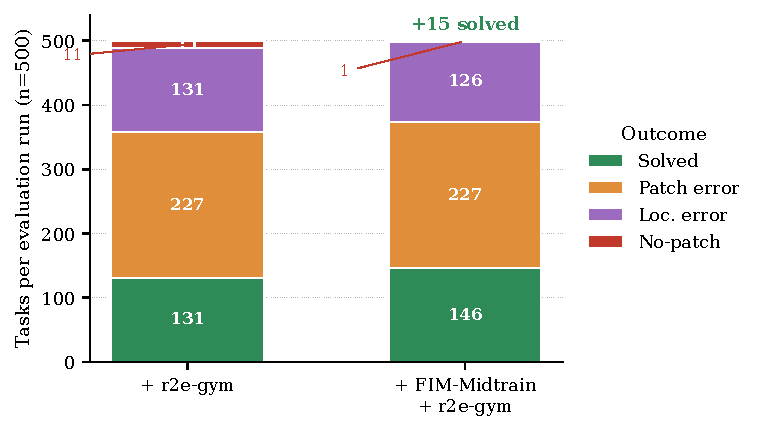
\includegraphics[width=0.55\linewidth]{figs/failure_modes.pdf}
\caption{Outcome distribution per evaluation run on SWE-Bench-Verified
(14B, R2E-Gym), averaged over three runs. Mid-training collapses the
no-patch failure mode ($\sim\!11 \to \sim\!1$ tasks per run) and adds
$+15$ solved tasks on average; localization and patch errors move only
slightly.}
\label{fig:failure_app}
\end{figure}

\subsection{No-Patch Mode: Mechanism}
\label{app:behavior_extra:nopatch}

The baseline no-patch failures recovered by mid-training are distributed
across all task buckets and are not concentrated in any single
repository. In every recovered case the baseline emitted
\texttt{<finish>} without applying any \texttt{str\_replace}, while ours
applied at least one edit. We interpret this as a direct consequence of
the fill-in-the-middle training signal: under FIM the model is always
conditioned to produce a non-empty token span between the prefix and
suffix, and we observe that this disposition survives the post-training
pipeline.

\subsection{Multi-File Tasks Are Not Differentially Helped}
\label{app:behavior_extra:multifile}

On the $71$ Verified tasks whose gold patch spans $\ge 2$ files, both
checkpoints solve $\sim\!11.3\%$ on average, and per-instance head-to-head
on this bucket is balanced. We attribute this to a mismatch in
granularity: our function-aware FIM mid-training operates at the
function level within files, so cross-file coordination is not directly
trained for. Extending the selection algorithm to cross-file function
pairs is a natural follow-up.

\subsection{A Concrete Contrast}
\label{app:behavior_extra:contrast}

The shift in termination behavior is clearest on cases where the
baseline quits prematurely. On \texttt{scikit-learn-26323}, for instance,
the baseline trajectory runs for a single step in every run, immediately
emits \texttt{<finish>} with an empty edit and the wrong target file,
and is scored as a failure; on the same task our agent runs $\sim\!41$
steps, applies on the order of $20$ \texttt{str\_replace} operations,
observes multiple negative tool returns, and recovers to a passing
patch. Pooling across the three runs, on the order of $\sim\!16$ of the
$\sim\!55$ tasks that ours uniquely solves on Verified have this
signature: the baseline emits \texttt{<finish>} with zero file overlap
with the gold patch (often before any negative observation has even
arrived), while ours iterates past intermediate signals and converges on
a correct edit. Mid-training does not enable a categorically new
capability on these instances; it changes the agent's stopping policy.